% Vorgaben Assignment aus Studienheft SQL03
% Formatvorgaben fuer den Text
% Umfang: 8 - 10 Seiten (inkl. Abbildungen und Tabellen, aber ohne Deckblatt, % Gliederung und Literaturverzeichnis, Eidesstattliche Erklaerung)
% Zeilenabstand: 1,5
% Schriftart: frei
% Schriftgrad: 12 pt
% Variablen, physikalische Groessen und Funktionszeichen werden kursiv gedruckt.
% Korrekturrand: links: 4,5 cm, rechts 2,0 cm, oben und unten jeweils 3,0 cm
% Deckblatt: (Adresse, AKAD-E-Mail-Adresse, Immatrikulationsnummer, Modul-
% bezeichnung, Thema, Datum, Felder für Korrektor)
% Gliederung (1 Seite)
% Literaturverzeichnis (3 - 5 Literaturquellen  z. B. Lehrbuecher, aktuelle Fachartikel recherchieren)
% Eidesstattliche Erklaerung (unterschrieben und fest eingebunden)
% Bearbeitungsdauer: 2 Monate


%
%% Document Class (Koma Script) -----------------------------------------
%% Doc: scrguien.pdf
\documentclass[%
   %draft=true,     % draft mode (no images, layout errors shown)
   draft=false,     % final mode 
%%% --- Paper Settings ---
   paper=a4,% [Todo: add alternatives]
   paper=portrait, % landscape
   pagesize=auto, % driver
%%% --- Base Font Size ---
   fontsize=12pt,%
%%% --- Koma Script Version ---
   version=last, %
%%% --- Global Package Options ---
   ngerman, % language (passed to babel and other packages)
            % (ngerman, english, french, ...)
]{scrreprt} % Classes: scrartcl, scrreprt, scrbook\usepackage[ngerman]{babel}

\newif\ifappendix
\newif\iflistoffigures
\newif\iflistoftables
\newif\ifacronym
\newif\iflistofformeln
\newif\ifassignment
\newif\ifabschlussarbeit

% Einstellungen für das Gesamtdokument
%Titel
\newcommand*{\Titel}{Thema des Assignments} 

%Betreff
\newcommand*{\Arbeitstyp}{Assignment im Modul ABC01} 

% Akademischer Grad
\newcommand*{\Grad}{Master of Science (M.Sc.)} 

%Betreuer
\newcommand*{\Betreuer}{Prof. Dr. Mustermann} 

%Vor- und Nachname
\newcommand*{\Name}{Max Mustermann}

%Straße und Hausnummer
\newcommand*{\Strasse}{Musterstr. 1a} 

%Plz und Ort
\newcommand*{\PlzOrt}{12345 Musterhausen} 

%Immatrikulationsnummer
\newcommand*{\Immatrikulationsnummer}{123456}

%Bearbeitungszeit
\newcommand*{\Bearbeitungszeit}{8 Wochen}

%Studiengang
\newcommand*{\Studiengang}{IT-Management}

%Email 
\newcommand*{\Email}{max.mustermann@akad.de} 

%PDF Beschreibung
\newcommand*{\pdfsubject}{Eine kurze Beschreibung, worum es geht}

%PDF Keywords
\newcommand*{\pdfkeywords}{akad, assignment, meta, information, pdf, hyperref, latex}


%(Wenn nicht benötigt, Zeile mit % auskommentieren oder löschen)

%% Anhang 
\appendixtrue

%% Verzeichnisse 
%
%% Abbildungsverzeichnis 
\listoffigurestrue
%% Tabellenverzeichnis
\listoftablestrue
%% Abkürzungsverzeichnis
\acronymtrue
%% Formelverzeichnis
%\listofformelntrue

%% Wird Vorlage für Assignment benutzt
\assignmenttrue


% Allgemeine Präambel für die Einbindung von Paketen
\usepackage[nottoc]{tocbibind} % Anzeigen des Literaturverzeichnisses im TOC
\usepackage{epsfig}
%\usepackage{times}
\usepackage{babel}
\usepackage{supertabular}
\usepackage{wrapfig}
\usepackage{multirow}
\usepackage[onehalfspacing]{setspace}
\usepackage{listings}
\usepackage{mathptmx}
\usepackage{geometry}
\usepackage{helvet}
\usepackage{courier}
\usepackage{setspace}
\usepackage{textcomp}
\usepackage[T1]{fontenc}
\usepackage[utf8]{inputenc}
\usepackage{float} % Notwendig fuer figure[h]
\usepackage[german=quotes]{csquotes}
\usepackage[style=alphabetic]{biblatex} % alternative: iso-authoryear
\usepackage{pdfpages}
% Fuer Schriftart Arial
%\usepackage[scaled]{uarial}

% Installation der Arial Schriftart unter Linux.
% wget http://tug.org/fonts/getnonfreefonts/install-getnonfreefonts
% texlua install-getnonfreefonts
% getnonfreefonts -r
% getnonfreefonts arial-urw


%% Einstellungen fuer Quellcode Highlighting

\usepackage{listings}
\usepackage{color}

\definecolor{mygreen}{rgb}{0,0.6,0}
\definecolor{mygray}{rgb}{0.5,0.5,0.5}
\definecolor{mymauve}{rgb}{0.58,0,0.82}

\lstset{ %
  backgroundcolor=\color{white},   % choose the background color; you must add \usepackage{color} or \usepackage{xcolor}
  basicstyle=\footnotesize,        % the size of the fonts that are used for the code
  breakatwhitespace=false,         % sets if automatic breaks should only happen at whitespace
  breaklines=true,                 % sets automatic line breaking
  captionpos=b,                    % sets the caption-position to bottom
  commentstyle=\color{mygreen},    % comment style
  deletekeywords={...},            % if you want to delete keywords from the given language
  escapeinside={\%*}{*)},          % if you want to add LaTeX within your code
  extendedchars=true,              % lets you use non-ASCII characters; for 8-bits encodings only, does not work with UTF-8
 % frame=single,                    % adds a frame around the code
  keepspaces=true,                 % keeps spaces in text, useful for keeping indentation of code (possibly needs columns=flexible)
  keywordstyle=\color{blue},       % keyword style
  language=Octave,                 % the language of the code
  morekeywords={*,...},            % if you want to add more keywords to the set
  numbers=left,                    % where to put the line-numbers; possible values are (none, left, right)
  numbersep=5pt,                   % how far the line-numbers are from the code
  numberstyle=\tiny\color{mygray}, % the style that is used for the line-numbers
  rulecolor=\color{black},         % if not set, the frame-color may be changed on line-breaks within not-black text (e.g. comments (green here))
  showspaces=false,                % show spaces everywhere adding particular underscores; it overrides 'showstringspaces'
  showstringspaces=true,          % underline spaces within strings only
  showtabs=true,                  % show tabs within strings adding particular underscores
  stepnumber=1,                    % the step between two line-numbers. If it's 1, each line will be numbered
  stringstyle=\color{mymauve},     % string literal style
  tabsize=2,                       % sets default tabsize to 2 spaces
  title=\lstname,                   % show the filename of files included with \lstinputlisting; also try caption instead of title
  belowskip= 0pt 
}

% PDF Einstellungen für Verlinkungen

\usepackage[
	pdftitle={\Titel},
	pdfsubject={\pdfsubject},
	pdfauthor={\Name},
	pdfkeywords={\pdfkeywords}
	hyperfootnotes=false,
	colorlinks=true,
	linkcolor=black,
	urlcolor=black,
	citecolor=black
]{hyperref}

%%% Abkürzungsverzeichnis
%\usepackage[
%%	footnote,	% Full names appear in the footnote
%%	smaller,		% Print acronym in smaller fontsize (required package: relsize)
%	printonlyused, % Print only acronyms that are actually used in the text
%%	dua, % print full names everytime
%%	nolist, % no list with all acronyms
%%	nohyperlinks, % no hyperlinks (required package: hyperref)
%]{acronym}

%%% Abkürzungsverzeichnis (Glossar) Neues Paket (kann nomencl und acronym ersetzen)
% muss nach hyperref eingebunden werden, um das Paket zu nutzen
% Abkürzungen werden nur im Glossar angezeigt, wenn sie im Dokument mindestens einmal genutzt wurden
\usepackage[
%	style=long,
	toc, % Glossar erscheint im Inhaltsverzeichnis
%	acronym, % Setzt Akronyme in ein gesondertes Verzeichnis
%	footnote, % Setzt eine Fußnote beim ersten verwendet wird
%	nomain,
%	style=altlist,
	nopostdot, % löscht den schlusspunkt nach jeder description
]{glossaries}
\glossarystyle{super}
\makeglossaries % Glossar generieren

\newfloat{Formel}{H}{for}

\renewcommand\UrlFont{\color{black}\rmfamily\itshape}

\renewcommand{\familydefault}{\rmdefault}
\newcommand{\bflabel}[1]{\normalfont{\normalsize{#1}}\hfill}

% Sonstige Hilfsfunktionen
%% Definition for Codeschnipsel im Fließtext
\newcommand{\code}{\texttt}

%% Todos mithilfe eines Rahmens hervorheben
\newcommand{\todo}[1]{\fbox{\parbox{\textwidth}{\textbf{To do:} #1}}}




% Style Einstellungen
%% Für Codeblöcke mit Syntax-Highlighting
%% http://www.ctan.org/tex-archive/macros/latex/contrib/minted/
%% Einkommentieren fuer Minted Syntax Highlighting
%\usepackage{minted}
%\definecolor{bg}{rgb}{0.95,0.95,0.95}

\makeatother

\ifassignment
\geometry{a4paper, left=25mm, right=20mm, top=30mm, bottom=30mm}
\else
\geometry{a4paper, left=45mm, right=20mm, top=30mm, bottom=30mm}
\fi

\pagenumbering{roman}


\usepackage[automark,headsepline]{scrlayer-scrpage}

\clearpairofpagestyles
\cfoot[\pagemark]{\pagemark}
\lehead{\headmark}
\rohead{\headmark}

\pagestyle{scrheadings}

% BEGIN DOCUMENT %%%%%%%%%%%%%%%%%%%%%%%%%%%%%%%%%%%%%%%%%%%%%%%%%%%%%%%%%%%%%%%
\begin{document}
%%%%%%%%%%%%%%%%%%%%%%%%%%%%%%%%%%%%%%%%%%%%%%%%%%%%%%%%%%%%%%%%%%%%%%%%%%%%%%%%

% TITEL PAGE %%%%%%%%%%%%%%%%%%%%%%%%%%%%%%%%%%%%%%%%%%%%%%%%%%%%%%%%%%%%%%%%%%%

\begin{titlepage}
\newgeometry{left=25mm, right=20mm, top=30mm, bottom=30mm}
\begin{center}
\thispagestyle{empty}

\Huge{\Titel}
\vspace{2cm}
\onehalfspacing

\Large{\textbf{\Arbeitstyp}}

\vspace{1cm}
\normalsize

von

\vspace{.5cm} 
\large{\Name}
\normalsize
\vspace{1cm}

\ifassignment
\else
Zur Erlangung des akademischen Grades \\
\textbf{\Grad}
\vspace{1cm}
\fi

Im Studiengang \Studiengang \\
an der staatlich anerkannten AKAD Hochschule Stuttgart
\vspace{2cm}

\today

\vspace{2cm}


\includegraphics[scale=0.35]{img/akad_logo.png}

\end{center}

\vfill
\begin{spacing}{1.2}
    \begin{tabbing}
	    \hspace{9cm}     \= \kill
	    \textbf{Bearbeitungszeit}  \>  \Bearbeitungszeit \\
	    \textbf{Betreuer}              \>  \Betreuer \\
	    \textbf{Immatrikulationsnummer}  \>  \Immatrikulationsnummer \\
	    \textbf{E-Mail}		\> \href{mailto:\Email}{\Email} \\
	    \textbf{Adresse}		\> \Strasse \\
	    		\> \PlzOrt
	\end{tabbing}
\end{spacing}
\restoregeometry
\end{titlepage}

%%%%%%%%%%%%%%%%%%%%%%%%%%%%%%%%%%%%%%%%%%%%%%%%%%%%%%%%%%%%%%%%%%%%%%%%%%%%%%%%

\clearpage

\normalsize

\begin{spacing}{1.0} % Verzeichnisse werden mit einzeiligem Abstand gesetzt
\newpage

% Inhaltsverzeichnis %%%%%%%%%%%%%%%%%%%%%%
\tableofcontents 
\newpage

% Abbildungsverzeichnis %%%%%%%%%%%%%%%%%%%%%%
\iflistoffigures
\listoffigures 
\newpage
\fi

% Tabellenverzeichnis %%%%%%%%%%%%%%%%%%%%%%
\iflistoftables
\listoftables 
\newpage
\fi

% Abkürzungsverzeichnis %%%%%%%%%%%%%%%%%%%%%%
\ifacronym
\chapter*{Abkürzungsverzeichnis}
\addcontentsline{toc}{chapter}{Abkürzungsverzeichnis} 


%% Hier Abkürzungen angeben
\begin{acronym}[ABK]
	\acro{Abk}{Abkürzungen}
	\acro{Test}{Wird nicht im Text verwendet und taucht auch nicht im Verzeichnis auf}
\end{acronym}

\fi

% Formelverzeichnis %%%%%%%%%%%%%%%%%%%%%%
\iflistofformeln
\listof{Formel}{Formelübersicht}
\newpage
\fi


\end{spacing} 

\clearpage

\newcounter{romanPagenumber} 
\setcounter{romanPagenumber}{\value{page}} % Roemische Seitenanzahl speichern.

\nocite{*} 

\pagenumbering{arabic}

\begin{spacing}{1.5} % Zeilenabstand: 1,5 fuer den Textteil

% Einleitung
\chapter{Einleitung}
\section{Einführung in das Thema}
Lorem ipsum dolor sit amet, consetetur sadipscing elitr, sed diam nonumy eirmod tempor invidunt ut labore et dolore magna aliquyam erat, sed diam voluptua. At vero eos et accusam et justo duo dolores et ea rebum. Stet clita kasd gubergren, no sea takimata sanctus est Lorem ipsum dolor sit amet. Lorem ipsum dolor sit amet, consetetur sadipscing elitr, sed diam nonumy eirmod tempor invidunt ut labore et dolore magna aliquyam erat, sed diam voluptua. At vero eos et accusam et justo duo dolores et ea rebum. Stet clita kasd gubergren, no sea takimata sanctus est Lorem ipsum dolor sit amet.

\section{Problemstellung und Ziel dieser Arbeit}

Lorem ipsum dolor sit amet, consetetur sadipscing elitr, sed diam nonumy eirmod tempor invidunt ut labore et dolore magna aliquyam erat, sed diam voluptua. At vero eos et accusam et justo duo dolores et ea rebum. Stet clita kasd gubergren, no sea takimata sanctus est Lorem ipsum dolor sit amet. Lorem ipsum dolor sit amet, consetetur sadipscing elitr, sed diam nonumy eirmod tempor invidunt ut labore et dolore magna aliquyam erat, sed diam voluptua. At vero eos et accusam et justo duo dolores et ea rebum. Stet clita kasd gubergren, no sea takimata sanctus est Lorem ipsum dolor sit amet.

\section{Aufbau der Arbeit}

\todo{An die fertige Arbeit anpassen}

Lorem ipsum dolor sit amet, consetetur sadipscing elitr, sed diam nonumy eirmod tempor invidunt ut labore et dolore magna aliquyam erat, sed diam voluptua. At vero eos et accusam et justo duo dolores et ea rebum. Stet clita kasd gubergren, no sea takimata sanctus est Lorem ipsum dolor sit amet. Lorem ipsum dolor sit amet, consetetur sadipscing elitr, sed diam nonumy eirmod tempor invidunt ut labore et dolore magna aliquyam erat, sed diam voluptua. 


%Grundlagen
\chapter{Grundlagen}
\section{Text}
Das ist eine \ac{abk}, die bei der zweiten Verwendung nur noch in der Kurzform \ac{abk} angezeigt wird.

\subsection{Fett}
\textbf{Lorem ipsum dolor sit amet, consetetur sadipscing elitr, sed diam nonumy eirmod tempor invidunt ut labore et dolore magna aliquyam erat, sed diam voluptua.}

\subsection{Kursiv}
\textit{Lorem ipsum dolor sit amet, consetetur sadipscing elitr, sed diam nonumy eirmod tempor invidunt ut labore et dolore magna aliquyam erat, sed diam voluptua.}

\subsection{Unterstrichen}
orem ipsum \underline{dolor} sit amet, consetetur sadipscing elitr, sed diam nonumy eirmod \underline{tempor} invidunt ut labore et dolore magna \underline{aliquyam} erat, sed diam voluptua.

\section{Fußnote}

Text mit Fußnote \footnote{Die Fußnote zum Text} 

\section{Zitate}

Dies ist ein ganz kurzer Beispieltext \footnote{\cite{Baeumle-Courth2004}}. Und noch ein weites Zitat \footnote{\cite{Torvalds2001}}
\\
Zitate auf Webseiten \footnote{\cite{gabler:individualsoftware}} \footnote{\cite{gabler:standardsoftware}}
\\
http://www.literatur-generator.de/

\section{Aufzählung}

\begin{itemize}
\item\textit{Punkt 1:} Text
\item Punkt 2: Text
\item Punkt 3: \\ Text
\end{itemize}

\section{Abkürzungen}
Hier werden \ac{Abk} aus dem Verzeichnis aufgerufen und gleich nochmal die gleiche \ac{Abk}.

%Hauppteil
\chapter{Hauptteil}

\section{Tabelle}

\begin{center}
\tablehead{ \textbf{Head1} & \textbf{Head2} & \textbf{Head3}
\\ }
\bottomcaption[Beschreibung]{Beschreibung. Quelle: Berger, Vorlesung, 2012, München }
\begin{supertabular}{c|c|c}
\hline
1 & 2 & 3 \\
4 & 5 & 6 \\
7 & 8 & 9 \\
1 & 2 & 3 \\
4 & 5 & 6 \\
7 & 8 & 9 \\
\end{supertabular}
\end{center}

\section{Bilder}

\begin{figure}[H]
\begin{center}
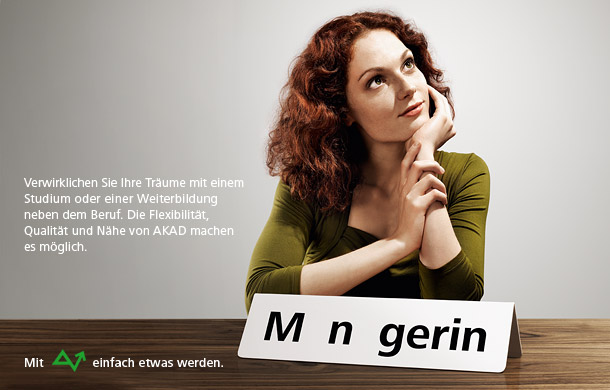
\includegraphics[scale=0.5]{img/akad_bild1.jpg}
\caption[Akad]{Akad. Quelle: www.akad.de}
\end{center}
\end{figure}

%%Einkommentieren fuer Syntax Highlighting. In vorlage.tex muessen auch 2 Zeilen einkommentiert werden
%\subsection{Syntax Highlighting}
%\begin{figure}[h]
%\begin{minted}[linenos=true,bgcolor=bg]{php}
%<?php 
%$title="Lorem";
%$desc = "Lorem Ipsum";
%include($_SERVER['DOCUMENT_ROOT'].'/header.php'); 
%?>
%\end{minted}
%\caption{Quellcode: Aufruf von header.php (PHP)}
%\label{abb:header}
%\end{figure}

\section{Formeln}

\begin{Formel}
$a+b=c$
\caption{AB Formel}
\end{Formel}


\section{Quellcode}
\begin{figure}[H]
\begin{lstlisting}[language=bash]
echo "Hello World"
\end{lstlisting}
\caption{Bash Hello World}
\end{figure}



%Schluss
\chapter{Bewertung}

\section{Zusammenfassung}
Lorem ipsum dolor sit amet, consetetur sadipscing elitr, sed diam nonumy eirmod tempor invidunt ut labore et dolore magna aliquyam erat, sed diam voluptua. At vero eos et accusam et justo duo dolores et ea rebum. Stet clita kasd gubergren, no sea takimata sanctus est Lorem ipsum dolor sit amet.

\section{kritische Würdigung}
Lorem ipsum dolor sit amet, consetetur sadipscing elitr, sed diam nonumy eirmod tempor invidunt ut labore et dolore magna aliquyam erat, sed diam voluptua. At vero eos et accusam et justo duo dolores et ea rebum. Stet clita kasd gubergren, no sea takimata sanctus est Lorem ipsum dolor sit amet.

\section{Ausblick}
Lorem ipsum dolor sit amet, consetetur sadipscing elitr, sed diam nonumy eirmod tempor invidunt ut labore et dolore magna aliquyam erat, sed diam voluptua. At vero eos et accusam et justo duo dolores et ea rebum. Stet clita kasd gubergren, no sea takimata sanctus est Lorem ipsum dolor sit amet.

\section{Erfolgsfaktoren}
Lorem ipsum dolor sit amet, consetetur sadipscing elitr, sed diam nonumy eirmod tempor invidunt ut labore et dolore magna aliquyam erat, sed diam voluptua. At vero eos et accusam et justo duo dolores et ea rebum. Stet clita kasd gubergren, no sea takimata sanctus est Lorem ipsum dolor sit amet.

\end{spacing}

\clearpage

\pagestyle{plain}


% Anhang 
\ifappendix
\appendix
\chapter{Anhang}

\begin{figure}[H]
\begin{center}
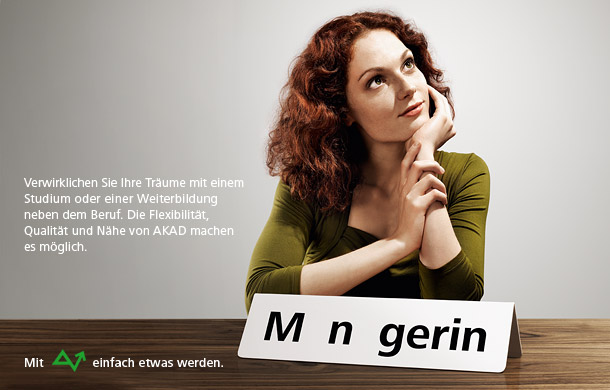
\includegraphics[scale=0.5]{img/akad_bild1.jpg}
\caption[Akad Anhang]{Akad Anhang. Quelle: www.akad.de}
\end{center}
\end{figure}

%\section{Example Appendix}
%\label{app:example}
%\includepdf[pages=-]{resources/example.pdf}
\clearpage
\fi

% Literaturverzeichniss - Ab hier wieder Roemische Seitenzahlen

\pagenumbering{roman}
\setcounter{page}{\theromanPagenumber}
\bibliographystyle{apalike}
\bibliography{literatur}
\onehalfspacing
\clearpage

\pagestyle{empty} 
\thispagestyle{empty}


\begin{center}
{\Large Eidesstattliche Erkl"arung}
\vspace*{4cm}\end{center}
\noindent
Ich versichere, dass ich das beiliegende Assignment selbstst"andig verfasst, keine anderen als die angegebenen Quellen und Hilfsmittel benutzt sowie alle w"ortlich oder sinngem"a"s "ubernommenen Stellen in der Arbeit gekennzeichnet habe. 
\vspace{3cm}

\hspace{-0.8cm}
\rule[0.5ex]{6.5cm}{1pt}
\hspace{1.3cm}
\rule[0.5ex]{6.5cm}{1pt}
(Datum, Ort)
\hspace{6.3cm}(Unterschrift)

\clearpage

%Messbox zur Druckkontrolle:
\newcommand{\Messbox}[2]{% Parameters: #1=Breite, #2=Hoehe
\setlength{\unitlength}{1.0mm}%
\begin{picture}(#1,#2)%
\linethickness{0.05mm}%
\put(0,0){\dashbox{0.2}(#1,#2)%
{\parbox{#1mm}{%
\centering\footnotesize 
%{\bf MESSBOX}\\ 
Breite $ = #1 {\ mm}$\\
H\"ohe $ = #2 {\ mm}$
}}}\end{picture}
}

\begin{center}
\textbf{--- Druckgröße kontrollieren! ---}
\\
\Messbox{100}{50} % Angabe der Breite/Hoehe in mm
\\
\textbf{--- Diese Seite nach dem Druck entfernen! ---}
\end{center}


\end{document}

